% =============================================================
%  HVDC Load Flow — Report
%  Uses the shared American Terawatt report style.
%  Compile:  pdflatex loadflow.tex   (run twice for ToC / references)
% =============================================================
\documentclass[11pt,a4paper]{article}

% Shared style lives in the repo-level template folder
\usepackage[corporate]{../../template/attemplate}
\usepackage{multirow}

% TikZ libraries used by the configuration diagrams in Section 2
\usetikzlibrary{arrows.meta,positioning,calc,shapes.geometric,fit}

% ---- Report metadata ----------------------------------------
\reporttitle{HVDC Load Flow}
\reportsubtitle{DC power flow, current and losses for symmetrical monopole and bipole configurations}
\reportauthor{Eugen Starschich}
\reportdocnumber{ATW-REP-LF-001}
\reportrevision{0.9}
\reportstatus{Draft}
\reportdate{\today}
\reportconfidentiality{Confidential}

\begin{document}

\makecover

\revisionhistory{
  \revrow{0.1}{Sep. 8, 2026}{Eugen Starschich}{Initial document}
  \revrow{0.2}{Sep. 8, 2026}{Eugen Starschich}{Conductor temperature correction; four case columns; one-pole-out case specified by power}
  \revrow{0.3}{Sep. 8, 2026}{Eugen Starschich}{Reference case aligned with current design inputs (Chukar DMR)}
  \revrow{0.4}{Sep. 9, 2026}{Eugen Starschich}{Refocused on the physical description; implementation section removed}
  \revrow{0.5}{Sep. 10, 2026}{Eugen Starschich}{HVDC element notation applied ($U_{dpp}$, $U_{dpe}$, $I_{d}$)}
  \revrow{0.6}{Sep. 10, 2026}{Eugen Starschich}{DC-side notation figure added; voltages qualified by station}
  \revrow{0.7}{Sep. 10, 2026}{Eugen Starschich}{Bipole notation figure added; resistances and currents renamed to $R_{d,hv}$, $R_{d,dmr}$, $I_{d,dmr}$}
  \revrow{0.8}{Sep. 10, 2026}{Eugen Starschich}{Conductor table reference added; data basis corrected to DC at 20 $^{\circ}$C and all results recomputed}
  \revrow{0.9}{Sep. 10, 2026}{Eugen Starschich}{References moved from footnotes to a closing References section}
}

\newpage
\tableofcontents
\clearpage

% ---- Body ---------------------------------------------------
\section{Scope and conventions}

\subsection{Purpose}
This document describes the steady-state power flow of a point-to-point HVDC
link: Assuming the power to be defined at the AC terminal of the receiving end. Two HVDC topologies 
arrangements are covered --- the \textbf{symmetrical
monopole (SMP)} and the \textbf{bipole with a dedicated metallic return (BIP)}.

\subsection{Direction and reference conventions}
Power flows from the \textbf{rectifier} (sending station) to the
\textbf{inverter} (receiving station). Four conventions fix the problem:

\begin{enumerate}[label=(\arabic*)]
  \item \textbf{Power is defined at the receiving end}, at the AC terminals of
        the inverter station.
  \item \textbf{DC voltage is regulated at the rectifier DC terminals.} The
        nominal dc voltage $U_{dpe\_rec}$ is defined at the sending station and
        the receiving-end voltage comes out lower by the resistive drop of the line.
  \item \textbf{Converter station losses are a fraction of station throughput}, applied per station, rather than a fixed number of
        megawatts.
  \item \textbf{Conductor resistance is corrected to a design temperature.}
        Conductor data is quoted at 20\,$^{\circ}$C; the flow is evaluated at a
        conductor temperature stated separately, 75\,$^{\circ}$C by default.
\end{enumerate}

Conventions (1) and (2) sit at opposite ends of the line, which is what makes
the current an implicit rather than an explicit quantity: the sending-end power
depends on the line loss, the line loss depends on the current, and the current
depends on the sending-end power. Section~\ref{sec:solution} closes that loop
in one step instead of iterating.

\subsection{Conductor data}
The one genuine conversion concerns the conductor data. Conductor tables give
DC resistance per 1000\,ft --- the values used here are the \emph{DC @
20\,$^{\circ}$C} column of the Southwire ACSR bare conductor tables~[1] ---
so the factor
\[
  \frac{5280\ \mathrm{ft/mi}}{1000\ \mathrm{ft}} = 5.28
\]
converts specific resistance to $\Omega$/mi before multiplying by the line
length in miles.

\subsection{Notation}
Figures~\ref{fig:dc-notation} and~\ref{fig:bip-notation} show the signal notation on
the DC side, for the SMP and BIP topologies.

Each quantity carries the station it is measured at, $rec$ or $inv$. In the
bipole it carries the pole as well, $pos$ or $neg$, since each pole has its own
converter pair; the HV conductor and the DMR are distinguished in both the
resistances, $R_{d\_hv}$ and $R_{d\_dmr}$, and the currents, $I_{d\_hv}$ and
$I_{d\_dmr}$; and $U_{dmr}$ is the DMR potential at the station where the return
is not earthed. The relations in the sections that follow use the unqualified
symbol wherever a statement holds for either pole or for either station.

\begin{figure}[!ht]
  \centering
  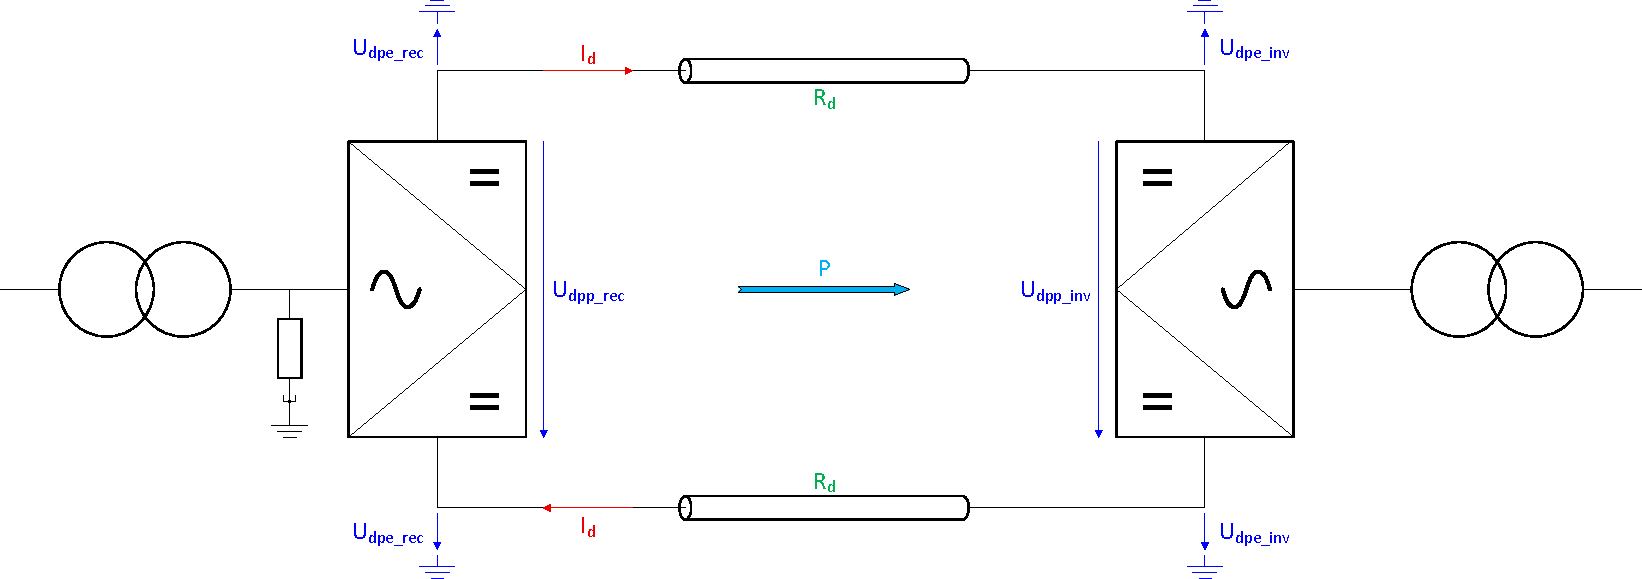
\includegraphics[width=\linewidth]{figures/dc-notation-smp.pdf}
  \caption{DC-side notation for SMP}
  \label{fig:dc-notation}
\end{figure}

\begin{figure}[!ht]
  \centering
  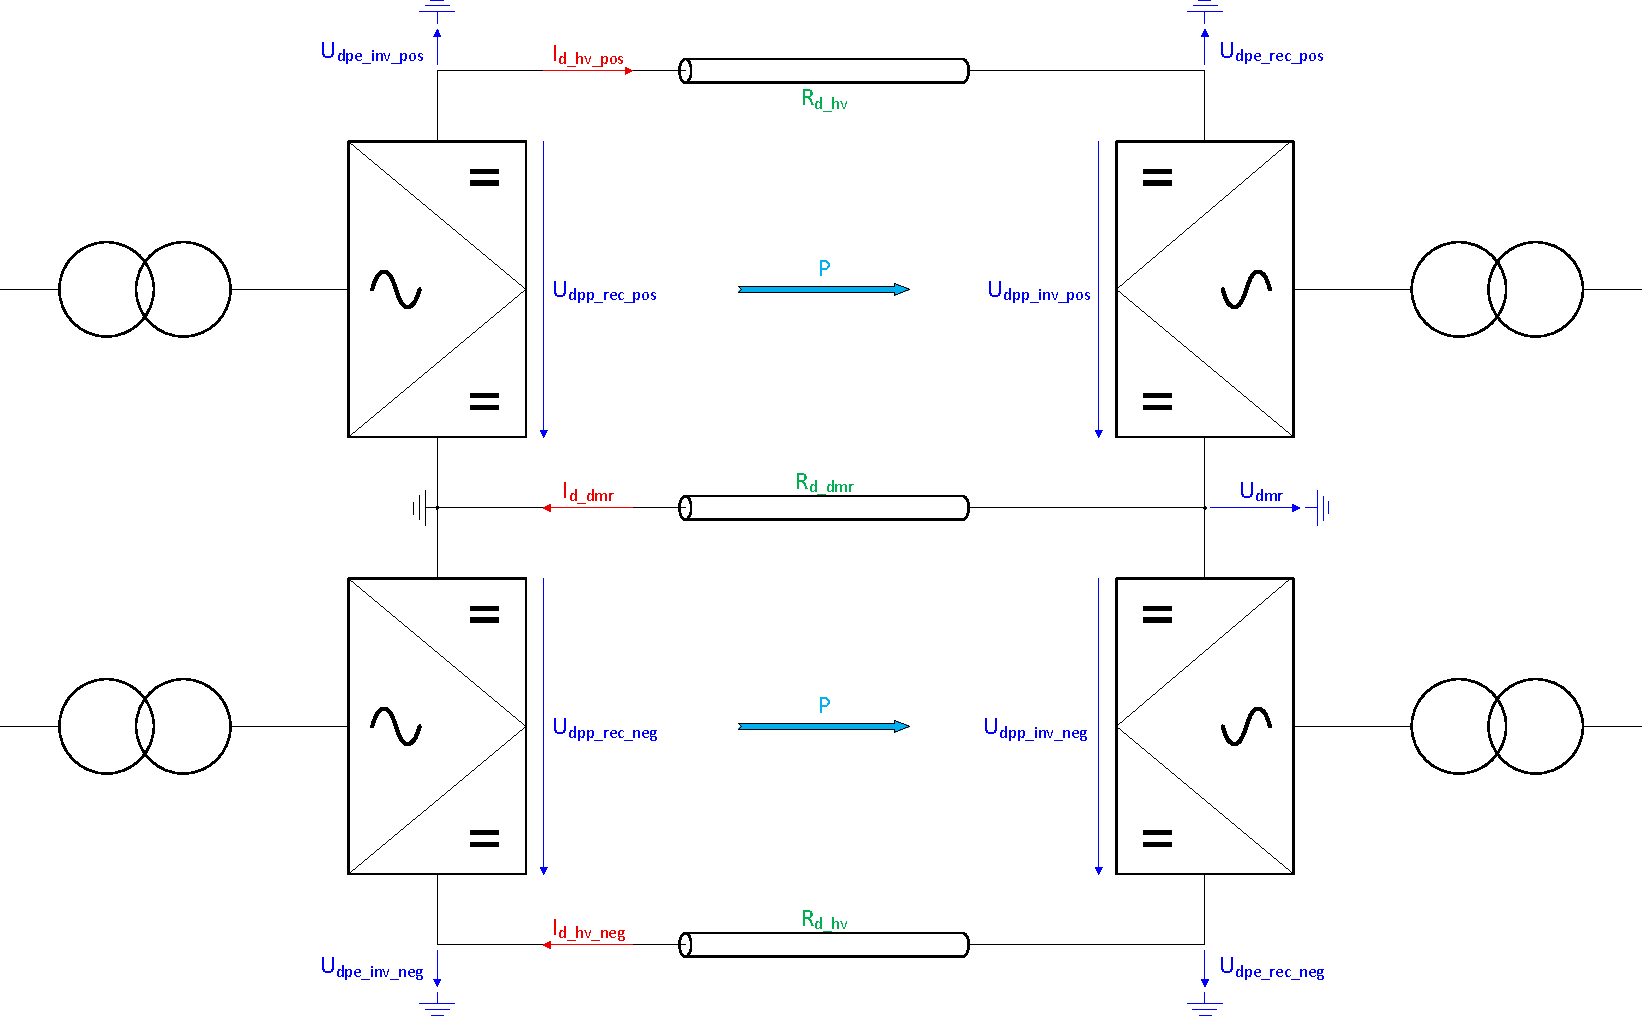
\includegraphics[width=\linewidth]{figures/dc-notation-bip.pdf}
  \caption{DC-side notation for BIP}
  \label{fig:bip-notation}
\end{figure}

\begin{table}[!ht]
  \centering
  \renewcommand{\arraystretch}{1.25}
  \begin{tabularx}{\linewidth}{@{}l l X@{}}
    \toprule
    \multicolumn{1}{c}{\textbf{Symbol}} & \multicolumn{1}{c}{\textbf{Unit}} & \textbf{Quantity} \\
    \midrule
    $P_{ac\_inv}$   & MW            & AC power at the receiving end (inverter AC terminals) --- \emph{given} \\
    $P_{ac\_rec}$   & MW            & AC power drawn at the sending end (rectifier AC terminals) \\
    $P_{dc\_inv}$   & MW            & DC power at the inverter DC terminals \\
    $P_{dc\_rec}$   & MW            & DC power at the rectifier DC terminals \\
    $U_{dpe}$      & kV            & DC pole-to-ground (earth) voltage \\
    $U_{dpe\_rec}$  & kV            & DC pole-to-ground voltage at the rectifier --- \emph{given} \\
    $U_{dpe\_inv}$  & kV            & DC pole-to-ground voltage at the inverter \\
    $U_{dpp}$      & kV            & DC voltage across a converter's DC terminals; $U_{dpp} = 2\cdot U_{dpe}$ for a symmetrical monopole \\
    $U_{dmr}$      & kV            & DMR potential at the station where the return is not earthed \\
    $U_{dpm\_inv}$  & kV            & DC pole-to-DMR voltage at the inverter (one pole out) \\
    $I_{d}$        & kA            & DC pole current, operating value \\
    $k$            & ---           & Number of energised poles: 2 normally, 1 with a pole out \\
    $L$            & mi            & DC line length \\
    $r'_{d\_hv}$      & $\Omega$/1000\,ft & Specific resistance of one HV subconductor \\
    $n_{hv}$       & ---           & Subconductors per pole (bundle count) \\
    $R_{d\_hv}$     & $\Omega$      & Resistance of one pole conductor over the whole length \\
    $r'_{d\_dmr}$     & $\Omega$/1000\,ft & Specific resistance of one DMR subconductor \\
    $n_{dmr}$      & ---           & Subconductors in the DMR bundle \\
    $R_{d\_dmr}$    & $\Omega$      & Resistance of the DMR over the whole length \\
    $I_{d\_dmr}$    & kA            & Current in the DMR; zero when the bipole is balanced \\
    $R_{loop}$     & $\Omega$      & Resistance of the complete current path (out and return) \\
    $T_{ref}$      & $^{\circ}$C   & Temperature the conductor resistance data refers to \\
    $T$            & $^{\circ}$C   & Conductor temperature the flow is evaluated at \\
    $T_{0}$        & $^{\circ}$C   & Inferred zero-resistance temperature of the conductor material \\
    $k_{T}$        & ---           & Temperature correction factor on the specific resistance \\
    $p_{rec}$      & ---           & Rectifier station loss fraction of throughput \\
    $p_{inv}$      & ---           & Inverter station loss fraction of throughput \\
    $P_{loss\_line}$& MW            & Total resistive loss of the DC line \\
    $\eta$         & ---           & Overall AC-to-AC efficiency of the link \\
    \bottomrule
  \end{tabularx}
  \caption{Notation.}
  \label{tab:notation}
\end{table}

\pagebreak

\section{Configurations covered}
\label{sec:configurations}

Figure~\ref{fig:configurations} shows the two arrangements the calculation
covers, and the current path each of them presents to the flow.

\begin{figure}[tbp]
  \centering
  \resizebox{\linewidth}{!}{%
  \begin{tikzpicture}[
    font=\scriptsize,
    conv/.style={draw=atFg, line width=0.6pt, fill=atBgSubtle, rounded corners=1pt,
                 align=center, inner sep=3pt, minimum width=11mm, minimum height=15mm},
    line/.style={draw=atFg, line width=1.1pt},
    dmr/.style={draw=atAccentFg, line width=1.1pt},
    idle/.style={draw=atFgSubtle, line width=1.1pt, dashed},
    ar/.style={draw=atFg, line width=1.1pt, -{Latex[length=1.8mm]}},
    lab/.style={font=\tiny, text=atFgMuted},
    acc/.style={font=\tiny, text=atAccentFg},
    ttl/.style={font=\small\bfseries, text=atFg},
  ]

  % ---------------- panel 1 : symmetrical monopole ----------------
  \node[ttl] at (3.1,2.35) {Symmetrical monopole};
  \node[conv] (r1) at (0.5,0.6) {REC};
  \node[conv] (i1) at (5.7,0.6) {INV};
  % positive and negative conductors
  \draw[ar] (1.06,1.25) -- (5.14,1.25);
  \draw[line] (5.14,-0.05) -- (1.06,-0.05);
  \node[lab, above] at (3.1,1.3) {$+V_d$ \quad $I_d$};
  \node[lab, below] at (3.1,-0.1) {$-V_d$ \quad $I_d$};
  \node[lab] at (3.1,0.6) {$R_{loop} = 2R_{HV}$};
  \draw[ar] (-0.7,0.6) -- (-0.1,0.6);
  \node[lab, left] at (-0.7,0.6) {$P_{ac,rec}$};
  \draw[ar] (6.3,0.6) -- (6.9,0.6);
  \node[lab, right] at (6.9,0.6) {$P_{ac,inv}$};
  \node[lab] at (3.1,-0.75) {$P_{dc} = 2 V_d I_d$};

  % ---------------- panel 2 : bipole with DMR ----------------
  \begin{scope}[xshift=9.6cm]
  \node[ttl] at (3.1,2.35) {Bipole with dedicated metallic return};
  \node[conv, minimum height=8mm] (rp) at (0.5,1.35) {REC$^+$};
  \node[conv, minimum height=8mm] (rn) at (0.5,-0.55) {REC$^-$};
  \node[conv, minimum height=8mm] (ip) at (5.7,1.35) {INV$^+$};
  \node[conv, minimum height=8mm] (in) at (5.7,-0.55) {INV$^-$};
  % pole conductors
  \draw[ar] (1.06,1.6) -- (5.14,1.6);
  \node[lab, above] at (3.1,1.65) {$+V_d$ \quad $I_d$ \quad $R_{HV}$};
  \draw[line] (5.14,-0.8) -- (1.06,-0.8);
  \node[lab, below] at (3.1,-0.85) {$-V_d$ \quad $I_d$ \quad $R_{HV}$};
  % DMR
  \draw[dmr] (1.06,0.4) -- (5.14,0.4);
  \node[acc, above] at (3.1,0.45) {DMR \quad $R_{DMR}$};
  \node[acc, below] at (3.1,0.35) {$I_{DMR} = 0$ when balanced};
  % station earths
  \draw[line] (0.5,0.95) -- (0.5,0.4);
  \draw[line] (0.5,-0.15) -- (0.5,0.4);
  \draw[line] (5.7,0.95) -- (5.7,0.4);
  \draw[line] (5.7,-0.15) -- (5.7,0.4);
  \node[lab] at (3.1,-1.45) {balanced: $P_{dc} = 2 V_d I_d$
                             \quad|\quad one pole out:
                             $P_{dc} = V_d I_d$, return through DMR};
  \end{scope}

  \end{tikzpicture}}
  \caption{The two conductor arrangements. In both normal cases the current
           path is a two-conductor loop of resistance $2R_{HV}$; only when a
           bipole pole is lost does the return move to the DMR and the loop
           resistance become $R_{HV}+R_{DMR}$.}
  \label{fig:configurations}
\end{figure}

\subsection{Symmetrical monopole}
The symmetrical monopole carries the full power on two conductors held at
$+V_{d}$ and $-V_{d}$ against ground, with no third conductor and no ground
path in service. The DC circuit is a single loop: current leaves the rectifier
on the positive conductor and returns on the negative one. The voltage seen by
the converter is therefore the pole-to-pole voltage $2V_{d}$, and
\[
  P_{dc} = 2\,V_{d}\,I_{d}.
\]
Because there is no return path other than the second conductor, the loss of
either conductor is the loss of the whole link --- there is no partial
operating mode, which is the reason a bipole is preferred where availability
matters.

\subsection{Bipole with dedicated metallic return}
The bipole runs two independently controlled poles at $\pm V_{d}$ plus a third,
lower-rated conductor: the dedicated metallic return. In normal
\textbf{balanced} operation the two pole currents are equal and opposite, the
DMR carries no current, and the circuit is electrically identical to the
symmetrical monopole:
\[
  P_{dc} = 2\,V_{d}\,I_{d},
  \qquad
  I_{DMR} = 0 .
\]
The DMR earns its place when the bipole becomes unbalanced. With one pole out
of service the remaining pole keeps operating and its current returns through
the DMR instead of the lost conductor, so the link continues at reduced
capacity. In that condition the circuit is a single-pole loop:
\[
  P_{dc} = V_{d}\,I_{d},
\]
and the return path resistance is that of the DMR rather than that of a second
HV bundle --- which is why the DMR conductor is a separate input in the
calculation, as it is generally not the same conductor as the poles.

\subsection{Reduced-capacity case as calculated}
The one-pole-out case can be posed two ways: hold the power and double the pole
current, or hold the current and accept roughly half the power. The workbook
takes the second --- the outage case runs at the \emph{same pole current} as
the balanced bipole, which keeps the case within the conductor and valve
ratings already established for normal operation and needs no separate rating
input. Power is then a result of that current, and comes out slightly below
half of the bipolar figure because the return path through the DMR is more
resistive than the parallel HV bundle it replaces.

\begin{table}[htbp]
  \centering
  \renewcommand{\arraystretch}{1.25}
  \begin{tabularx}{\linewidth}{@{}l c c X@{}}
    \toprule
    \textbf{Configuration} & \textbf{$P_{dc}$} & \textbf{$R_{loop}$} &
    \textbf{Current path} \\
    \midrule
    Symmetrical monopole
      & $2 V_{d} I_{d}$ & $2 R_{HV}$
      & Out on the positive conductor, back on the negative conductor. \\
    Bipole, balanced
      & $2 V_{d} I_{d}$ & $2 R_{HV}$
      & Out on the positive pole, back on the negative pole; DMR idle. \\
    Bipole, one pole out
      & $V_{d} I_{d}$ & $R_{HV} + R_{DMR}$
      & Out on the healthy pole, back through the DMR. \\
    \bottomrule
  \end{tabularx}
  \caption{The three cases carried in the Load Flow tab. The first two share
           the same equations; only the third involves the DMR.}
  \label{tab:cases}
\end{table}


\section{Model}
\label{sec:model}

The link is represented by three elements in series: the rectifier station, the
DC line, and the inverter station. Each is a single algebraic relation.

\subsection{Line resistance}
The resistance of one pole conductor over the whole route is the specific
resistance of a single subconductor, divided by the number of subconductors in
the bundle (they are electrically in parallel), converted to $\Omega$/mi and
multiplied by the length:
\begin{equation}
  R_{HV} = \frac{r'_{HV}\cdot 5.28}{n_{HV}}\; L ,
  \qquad
  R_{DMR} = \frac{r'_{DMR}\cdot 5.28}{n_{DMR}}\; L .
  \label{eq:resistance}
\end{equation}
The resistance that matters for the flow is that of the complete circuit ---
out and back --- which depends on the configuration:
\begin{equation}
  R_{loop} =
  \begin{cases}
    2\,R_{HV}          & \text{symmetrical monopole, and balanced bipole,}\\[2pt]
    R_{HV} + R_{DMR}   & \text{bipole with one pole out (DMR return).}
  \end{cases}
  \label{eq:loop}
\end{equation}

Equation~\eqref{eq:resistance} is a DC resistance at the temperature of the
underlying conductor table. No temperature correction, skin effect or
proximity effect is applied; on a DC line the first is the only one that
matters and it is handled by choosing the conductor data at the design
temperature (Section~\ref{sec:assumptions}).

\subsection{Converter stations}
Station losses are taken as a fraction of the power passing through the
station. The two stations therefore differ only in which side of the
conversion is known:
\begin{align}
  \text{rectifier (AC}\rightarrow\text{DC):} \quad
    & P_{dc,rec} = P_{ac,rec}\,\bigl(1-p_{rec}\bigr)
      \quad\Longleftrightarrow\quad
      P_{ac,rec} = \frac{P_{dc,rec}}{1-p_{rec}},
      \label{eq:rect}\\[2pt]
  \text{inverter (DC}\rightarrow\text{AC):} \quad
    & P_{ac,inv} = P_{dc,inv}\,\bigl(1-p_{inv}\bigr)
      \quad\Longleftrightarrow\quad
      P_{dc,inv} = \frac{P_{ac,inv}}{1-p_{inv}}.
      \label{eq:inv}
\end{align}
A single fraction lumps everything inside the station fence: valve conduction
and switching losses, converter transformer and reactor losses, cooling and
auxiliary supply. The loss fraction is a straight percentage of throughput, so
it scales linearly with power and does not capture the no-load component of a
real loss curve; see Section~\ref{sec:assumptions}.

Because power is specified at the receiving AC terminals,
Equation~\eqref{eq:inv} is the \emph{entry point} of the whole calculation: it
converts the given $P_{ac,inv}$ into the DC power that must arrive at the
inverter DC terminals.

\subsection{DC line}
With the DC voltage held at $V_{d}$ pole-to-ground at the rectifier, the power
leaving the rectifier and the resistive loss of the line are
\begin{equation}
  P_{dc,rec} = k\,V_{d}\,I_{d},
  \qquad
  P_{loss,line} = R_{loop}\,I_{d}^{\,2},
  \qquad
  k =
  \begin{cases}
    2 & \text{two poles energised,}\\
    1 & \text{one pole out,}
  \end{cases}
  \label{eq:dcline}
\end{equation}
and the power arriving at the inverter DC terminals is the difference:
\begin{equation}
  P_{dc,inv} = k\,V_{d}\,I_{d} - R_{loop}\,I_{d}^{\,2}.
  \label{eq:flow}
\end{equation}
Equation~\eqref{eq:flow} is the load flow equation of the link. Everything in
Section~\ref{sec:solution} follows from solving it.

The loss splits between the conductors in proportion to their resistances,
which is reported separately because the DMR contribution is what distinguishes
the outage case:
\begin{equation}
  P_{loss,HV} =
  \begin{cases}
    2R_{HV} I_{d}^{\,2} & \text{balanced,}\\
    R_{HV} I_{d}^{\,2}  & \text{one pole out,}
  \end{cases}
  \qquad
  P_{loss,DMR} =
  \begin{cases}
    0                    & \text{balanced,}\\
    R_{DMR} I_{d}^{\,2}  & \text{one pole out.}
  \end{cases}
  \label{eq:losssplit}
\end{equation}

\subsection{Receiving-end voltage}
The voltage at the far end of the line is the sending-end voltage less the drop
along the conductors the current actually traverses. With two poles energised
the arrangement is symmetric --- each conductor drops $I_{d}R_{HV}$ and the
midpoint stays at ground --- so the pole-to-ground voltage at the inverter is
\begin{equation}
  V_{d,inv} = V_{d} - I_{d}\,R_{HV}
  \qquad\text{(two poles energised),}
  \label{eq:vinv}
\end{equation}
which is consistent with Equation~\eqref{eq:flow}, since
$2V_{d,inv}I_{d} = 2V_{d}I_{d} - 2R_{HV}I_{d}^{2}$. With one pole out the whole
loop drop appears between the healthy pole and the DMR, so the corresponding
figure is a pole-to-DMR voltage:
\begin{equation}
  V_{d,inv} = V_{d} - I_{d}\,R_{loop}
  \qquad\text{(one pole out, pole-to-DMR).}
  \label{eq:vinvmono}
\end{equation}

\section{Solution of the load flow}
\label{sec:solution}

\subsection{Why the current is not explicit}
If both the power and the voltage were specified at the same end of the line,
the current would follow from a division. They are not: power is fixed at the
receiving end and voltage at the sending end, and the two are separated by a
loss that itself depends on the current. Substituting the target power into
Equation~\eqref{eq:flow} gives a quadratic in $I_{d}$ rather than a linear
relation. It is a quadratic that can be solved in closed form, so no iteration
is needed --- which is what keeps the calculation a single row of the
spreadsheet.

\subsection{Two poles energised (symmetrical monopole, balanced bipole)}
Start from the required DC power at the inverter, Equation~\eqref{eq:inv}:
\begin{equation}
  P_{dc,inv} = \frac{P_{ac,inv}}{1-p_{inv}} .
  \label{eq:step1}
\end{equation}
Insert it into Equation~\eqref{eq:flow} with $k=2$ and collect terms:
\begin{equation}
  R_{loop}\,I_{d}^{\,2} - 2 V_{d}\,I_{d} + P_{dc,inv} = 0 .
  \label{eq:quadratic}
\end{equation}
The roots are
\[
  I_{d} = \frac{2V_{d} \pm \sqrt{4V_{d}^{2} - 4R_{loop}P_{dc,inv}}}{2R_{loop}}
        = \frac{V_{d} \pm \sqrt{V_{d}^{2} - R_{loop}P_{dc,inv}}}{R_{loop}},
\]
and the operating point is the \textbf{lower} root:
\begin{equation}
  \boxed{\;
  I_{d} = \frac{V_{d} - \sqrt{V_{d}^{2} - R_{loop}\,P_{dc,inv}}}{R_{loop}}
  \;}
  \label{eq:current}
\end{equation}
with $V_{d}$ in kV, $R_{loop}$ in $\Omega$, $P_{dc,inv}$ in MW and $I_{d}$ in
kA.

Both roots deliver the same power to the inverter, but they do it at different
efficiencies: the upper root is the high-current solution on the far side of
the line's maximum power point, where more current is pushed through the line
only to burn the extra in $I^{2}R$. It is not an operating point any converter
control would choose, and it lies far outside the current rating of the
conductors. The lower root is the physical one.

\subsection{Maximum transferable power}
The square root in Equation~\eqref{eq:current} becomes imaginary when the
requested power exceeds what the line can deliver at that voltage. The limit
follows from $\mathrm{d}P_{dc,inv}/\mathrm{d}I_{d} = 0$ applied to
Equation~\eqref{eq:flow}:
\begin{equation}
  I_{d}\big|_{P_{max}} = \frac{k\,V_{d}}{2R_{loop}},
  \qquad
  P_{max} = \frac{k^{2}V_{d}^{2}}{4R_{loop}} =
  \begin{cases}
    \dfrac{V_{d}^{2}}{R_{loop}}   & \text{two poles energised,}\\[6pt]
    \dfrac{V_{d}^{2}}{4R_{loop}}  & \text{one pole out.}
  \end{cases}
  \label{eq:pmax}
\end{equation}
$P_{max}$ is reported as a solvability check, not as a capability: at that
point half the sending-end power is dissipated in the line. For any sensible
design it sits an order of magnitude above the rating, and a real link is
limited by conductor thermal rating and valve current long before it. Its
practical use is diagnostic --- a \verb|#NUM!| in the current row means the
requested power, voltage and resistance combination has no solution, and
comparing against $P_{max}$ shows immediately which input is at fault.

\subsection{Forward chain}
With the current known, the rest of the quantities follow directly:
\begin{align}
  P_{dc,rec}      &= k\,V_{d}\,I_{d}                         &&\text{[Eq.~\eqref{eq:dcline}]} \label{eq:c1}\\
  P_{loss,line}   &= R_{loop}\,I_{d}^{\,2}                    &&\text{[Eq.~\eqref{eq:dcline}], split by Eq.~\eqref{eq:losssplit}} \label{eq:c2}\\
  V_{d,inv}       &= V_{d} - I_{d}R_{HV}                      &&\text{[Eq.~\eqref{eq:vinv}]} \label{eq:c3}\\
  P_{ac,rec}      &= \frac{P_{dc,rec}}{1-p_{rec}}             &&\text{[Eq.~\eqref{eq:rect}]} \label{eq:c4}\\
  P_{loss,total}  &= P_{ac,rec} - P_{ac,inv}                  &&\text{AC-to-AC loss} \label{eq:c5}\\
  \eta            &= \frac{P_{ac,inv}}{P_{ac,rec}}            &&\text{overall efficiency} \label{eq:c6}
\end{align}
The three loss contributions add up to the total, which is the closure check
built into the workbook:
\begin{equation}
  P_{ac,rec} - P_{ac,inv}
  = \underbrace{p_{rec}P_{ac,rec}}_{\text{rectifier}}
  + \underbrace{R_{loop}I_{d}^{\,2}}_{\text{line}}
  + \underbrace{p_{inv}P_{dc,inv}}_{\text{inverter}} .
  \label{eq:closure}
\end{equation}

\subsection{Bipole with one pole out}
The outage case is solved forward rather than backward, because the input is a
current and not a power. Taking the pole current from the balanced bipole
solution,
\begin{equation}
  I_{d,mono} = I_{d,bipole},
  \qquad
  R_{loop} = R_{HV} + R_{DMR},
  \label{eq:monoin}
\end{equation}
the chain runs in the opposite direction to Equation~\eqref{eq:step1}:
\begin{align}
  P_{dc,rec}    &= V_{d}\,I_{d} \label{eq:m1}\\
  P_{loss,line} &= R_{HV}I_{d}^{\,2} + R_{DMR}I_{d}^{\,2}
                 = R_{loop}I_{d}^{\,2} \label{eq:m2}\\
  P_{dc,inv}    &= P_{dc,rec} - P_{loss,line} \label{eq:m3}\\
  P_{ac,inv}    &= P_{dc,inv}\,\bigl(1-p_{inv}\bigr) \label{eq:m4}
\end{align}
so that the transferable power is a \emph{result} of the case rather than an
input. The residual capability is reported as a fraction of the bipolar
rating,
\begin{equation}
  \frac{P_{ac,inv,mono}}{P_{ac,inv,bipole}} ,
  \label{eq:ratio}
\end{equation}
which lands slightly below 50\,\% --- the pole current is unchanged but only
one pole carries power, and the DMR return is more resistive than the HV
bundle it replaces.

\subsection{Current margin}
The margin does not enter the flow. It scales the operating current to a rating
figure used for conductor selection, valve and bushing ratings, switchgear and
protection settings:
\begin{equation}
  I_{rated} = \bigl(1+m\bigr)\,I_{d}.
  \label{eq:margin}
\end{equation}
Losses, voltage drops and powers are all reported at the operating current
$I_{d}$, not at $I_{rated}$; the margined value is a sizing quantity only. If a
worst-case loss figure is wanted, the calculation is re-run with the power
input raised rather than by substituting $I_{rated}$ into the loss equation,
which would be inconsistent with the stated power.

\section{Worked cases}
\label{sec:reference}

\subsection{The cases}
Four operating cases are worked through below: the 1\,GW symmetrical monopole,
a double symmetrical monopole variant, the 3\,GW bipole, and that bipole
holding half its transfer on one pole. Station losses are 1.2\,\% per station
and the current margin 5\,\%. All conductor data is the DC resistance at
20\,$^{\circ}$C from the ACSR tables and the flow is evaluated at a conductor
temperature of 75\,$^{\circ}$C.

\begin{table}[t]
  \centering
  \small
  \renewcommand{\arraystretch}{1.25}
  \begin{tabularx}{\linewidth}{@{}X l r r r r@{}}
    \toprule
    \textbf{Given} & \textbf{Unit} &
    \textbf{SMP} & \textbf{DSMP} & \textbf{BIP} &
    \textbf{BIP 1 pole} \\
    \midrule
    AC power at receiving end     & MW                & 1{,}000 & 1{,}500 & 3{,}000 & 1{,}500 \\
    DC voltage pole-to-ground $U_{dpe,rec}$ & kV                & 400     & 400     & 525     & 525     \\
    DC line length                & mi                & 160     & 200     & 200     & 200     \\
    HV conductor                  & ---               & Bluebird & Chukar & Bluebird & Bluebird \\
    HV subconductors per pole     & ---               & 1       & 2       & 2       & 2       \\
    Specific HV resistance        & $\Omega$/1000\,ft & 0.00801 & 0.00970 & 0.00801 & 0.00801 \\
    DMR conductor                 & ---               & n/a     & n/a     & Chukar  & Chukar  \\
    DMR subconductors             & ---               & n/a     & n/a     & 2       & 1       \\
    Specific DMR resistance       & $\Omega$/1000\,ft & n/a     & n/a     & 0.00970 & 0.00970 \\
    Reference temperature $T_{ref}$ & $^{\circ}$C     & 20      & 20      & 20      & 20      \\
    Conductor temperature $T$     & $^{\circ}$C       & 75      & 75      & 75      & 75      \\
    Zero-resistance temperature $T_{0}$ & $^{\circ}$C & 228     & 228     & 228     & 228     \\
    Losses per converter station  & \%                & 1.2     & 1.2     & 1.2     & 1.2     \\
    Margin for DC current         & \%                & 5       & 5       & 5       & 5       \\
    \bottomrule
  \end{tabularx}
  \caption{Given quantities for the four cases. BIP\,1\,pole is the 3\,GW
           bipole with one pole out of service, on the same plant as the BIP
           case and with its own post-contingency transfer.}
  \label{tab:refinputs}
\end{table}

\subsection{Temperature correction and line resistance}
The correction factor is common to all four cases,
Equation~\eqref{eq:ktvalue}:
\[
  k_{T} = \frac{228+75}{228+20} = 1.2218 .
\]
Applying Equation~\eqref{eq:resistance} to the bipole, whose HV conductor and
length the outage case shares:
\[
  R_{d,hv} = \frac{0.00801\cdot 5.28}{2}\cdot 200 \cdot 1.2218
         = 4.229 \cdot 1.2218 = 5.167\ \Omega,
\]
and to the single-subconductor DMR that carries the return in the outage case:
\[
  R_{d,dmr} = \frac{0.00970\cdot 5.28}{1}\cdot 200 \cdot 1.2218
          = 10.243 \cdot 1.2218 = 12.515\ \Omega .
\]
So $R_{loop} = 10.335\,\Omega$ balanced and $17.682\,\Omega$ with the return
through the DMR. At the 20\,$^{\circ}$C data temperature those figures would
have been $8.459\,\Omega$ and $14.472\,\Omega$: the correction alone adds
22\,\% to every resistive loss reported below.

\subsection{Balanced bipole, step by step}
Following Section~\ref{sec:solution} with $k=2$:
\begin{align*}
  P_{dc,inv} &= \frac{3000}{1-0.012} = 3036.4\ \mathrm{MW}
              && \text{Eq.~\eqref{eq:step1}} \\
  I_{d}      &= \frac{525 - \sqrt{525^{2} - 10.335\cdot 3036.4}}{10.335}
              = \frac{525 - 494.21}{10.335} = 2.979\ \mathrm{kA}
              && \text{Eq.~\eqref{eq:current2}} \\
  P_{dc,rec} &= 2\cdot 525 \cdot 2.979 = 3128.2\ \mathrm{MW}
              && \text{Eq.~\eqref{eq:c1}} \\
  P_{loss,line} &= 10.335 \cdot 2.979^{2} = 91.7\ \mathrm{MW}
              && \text{Eq.~\eqref{eq:c2}} \\
  U_{dpe,inv}  &= 525 - 2.979\cdot 5.167 = 509.6\ \mathrm{kV}
              && \text{Eq.~\eqref{eq:vinv}} \\
  P_{ac,rec} &= \frac{3128.2}{1-0.012} = 3166.2\ \mathrm{MW}
              && \text{Eq.~\eqref{eq:c4}} \\
  \eta       &= \frac{3000}{3166.2} = 94.75\,\%
              && \text{Eq.~\eqref{eq:c6}}
\end{align*}
The loss balance of Equation~\eqref{eq:closure} closes:
$38.0 + 91.7 + 36.4 = 166.2\ \mathrm{MW} = P_{ac,rec}-P_{ac,inv}$.

\subsection{One pole out, step by step}
The same plant with $k=1$, the DMR in the loop, and its own 1500\,MW target:
\begin{align*}
  P_{dc,inv} &= \frac{1500}{1-0.012} = 1518.2\ \mathrm{MW} \\
  I_{d}      &= \frac{525 - \sqrt{525^{2} - 4\cdot 17.682\cdot 1518.2}}
                     {2\cdot 17.682}
              = \frac{525 - 410.16}{35.36} = 3.247\ \mathrm{kA}
              && \text{Eq.~\eqref{eq:current}} \\
  P_{dc,rec} &= 525 \cdot 3.247 = 1704.6\ \mathrm{MW} \\
  P_{loss,line} &= 5.167\cdot 3.247^{2} + 12.515\cdot 3.247^{2}
                 = 54.5 + 131.9 = 186.4\ \mathrm{MW}
              && \text{Eq.~\eqref{eq:losssplit}}
\end{align*}
Half the power, and yet a higher current and twice the line loss of the
balanced bipole. This is the case that sizes the conductor.

\subsection{Results}
Table~\ref{tab:refresults} collects the four cases, each at the
75\,$^{\circ}$C conductor temperature.

\begin{table}[t]
  \centering
  \small
  \renewcommand{\arraystretch}{1.25}
  \begin{tabularx}{\linewidth}{@{}X l r r r r@{}}
    \toprule
    \textbf{Result} & \textbf{Unit} &
    \textbf{SMP} & \textbf{DSMP} & \textbf{BIP} &
    \textbf{BIP 1 pole} \\
    \midrule
    Temperature correction factor    & ---      & 1.2218  & 1.2218  & 1.2218  & 1.2218  \\
    HV resistance per pole           & $\Omega$ & 8.268   & 6.257   & 5.167   & 5.167   \\
    DMR resistance                   & $\Omega$ & ---     & ---     & ---     & 12.515  \\
    Loop resistance                  & $\Omega$ & 16.535  & 12.515  & 10.335  & 17.682  \\
    DC power at inverter terminals   & MW       & 1{,}012.1 & 1{,}518.2 & 3{,}036.4 & 1{,}518.2 \\
    DC current, operating            & A        & 1{,}300 & 1{,}958 & 2{,}979 & 3{,}247 \\
    DC current, rated (5\,\% margin) & A        & 1{,}365 & 2{,}056 & 3{,}128 & 3{,}409 \\
    DC power at rectifier terminals  & MW       & 1{,}040.1 & 1{,}566.2 & 3{,}128.2 & 1{,}704.6 \\
    Line losses, HV conductors       & MW       & 27.9    & 48.0    & 91.7    & 54.5    \\
    Line losses, DMR                 & MW       & ---     & ---     & 0.0     & 131.9   \\
    Total DC line losses             & MW       & 27.9    & 48.0    & 91.7    & 186.4   \\
    DC voltage at inverter $U_{dpe,inv}$ & kV    & 389.3   & 387.7   & 509.6   & 508.2   \\
    DC voltage at inverter $U_{dpm,inv}$ & kV       & ---     & ---     & ---     & 467.6   \\
    AC power at sending end          & MW       & 1{,}052.7 & 1{,}585.2 & 3{,}166.2 & 1{,}725.3 \\
    Total losses, AC to AC           & MW       & 52.7    & 85.2    & 166.2   & 225.3   \\
    Overall efficiency               & \%       & 94.99   & 94.62   & 94.75   & 86.94   \\
    Maximum transferable power       & MW       & 9{,}676 & 12{,}785 & 26{,}671 & 3{,}897 \\
    \bottomrule
  \end{tabularx}
  \caption{Results at a conductor temperature of 75\,$^{\circ}$C.}
  \label{tab:refresults}
\end{table}

\subsection{Reading the results}
Four points are worth drawing out.

\textbf{The outage state sets the current rating.} At 3247\,A the bipole
holding half its transfer on one pole draws 9\,\% more current than it does at
full power on two, and with the margin applied it asks for 3409\,A against
3128\,A in normal operation. A conductor or valve sized on balanced operation
alone would be undersized for the contingency it exists to survive.

\textbf{The DMR dominates the outage loss.} 132\,MW of the 186\,MW lost in the
one-pole-out case is in the DMR alone, because a single Chukar subconductor is
2.4 times the resistance of the two-conductor Bluebird pole bundle it stands in
for. Doubling the DMR to two subconductors brings $R_{d,dmr}$ to
6.257\,$\Omega$, the current to 3101\,A and the line loss to 110\,MW --- a
76\,MW improvement for one extra conductor, and the first thing to settle in
the DMR design.

\textbf{Temperature is not a detail.} Every resistance and every line loss in
Table~\ref{tab:refresults} is 22\,\% higher than the conductor table suggests,
purely because the line is evaluated hot. Carried through to the bipole
efficiency the correction is worth about half a percentage point --- the same
order as the difference between the conductor options being compared, so a
comparison made at data temperature would not be a fair one.

\textbf{Where the power is defined changes the current.} Taken as the power
\emph{leaving} the rectifier over a line at data temperature, 3000\,MW on the
bipole corresponds to $P/(2\cdot U_{dpe,rec}) = 2857\,\mathrm{A}$. Required to
\emph{arrive} at the receiving AC terminals through a hot line, the same
3000\,MW needs 2979\,A, because the current now has to cover the line and
converter losses as well. The second figure is the one to size equipment
against when the transfer is guaranteed at the point of delivery.

\section{Assumptions and limitations}
\label{sec:assumptions}

\subsection{Assumptions}
Table~\ref{tab:assumptions} lists what the relations take for granted, and what
each assumption costs in accuracy.

\begin{table}[!ht]
  \centering
  \small
  \renewcommand{\arraystretch}{1.25}
  \begin{tabularx}{\linewidth}{@{}l X@{}}
    \toprule
    \multicolumn{1}{c}{\textbf{Assumption}} & \textbf{Consequence and justification} \\
    \midrule
    Purely resistive DC line
      & No inductance or capacitance appears in the relations. Correct for a
        steady-state DC flow; line charging and inductance matter only for
        transients and fault studies. \\
    Uniform conductor temperature
      & The whole route sits at the single design temperature $T$. In service
        the temperature varies with ambient, wind and loading along the line,
        so the reported loss is that of the stated design condition rather
        than of any particular hour. \\
    Linear resistance-temperature law
      & Equation~\eqref{eq:ktemp} is the standard inferred-zero-temperature
        form, accurate to well within a percent from ambient to the maximum
        continuous rating of an ACSR conductor. \\
    Aluminium carries the current
      & The steel core of an ACSR conductor is neglected in the resistance,
        which is standard practice; $T_{0} = 228\,^{\circ}$C is the aluminium
        constant. \\
    Station losses proportional to throughput
      & No no-load term, so light-load efficiency is overstated while
        full-load efficiency is representative.\\
    Balanced bipole carries no DMR current
      & The pole currents are taken as exactly equal. In service a small
        unbalance flows in the DMR; its loss contribution is second order,
        going with the square of a few percent of $I_{d}$. \\
    \bottomrule
  \end{tabularx}
  \caption{Assumptions underlying the load flow relations.}
  \label{tab:assumptions}
\end{table}

\subsection{Outside the scope}
The following are deliberately not treated here, each belonging to a dedicated
study:

\begin{itemize}\setlength{\itemsep}{0.3em}
  \item \textbf{Reactive power and AC-side voltage.} Only active power crosses
        the converter boundary in these relations. Converter reactive
        capability and AC network voltage support belong to the AC side of the
        design and, ultimately, to interconnection studies.
  \item \textbf{Thermal rating of the conductor.} The flow yields the current
        and assumes a conductor temperature; whether that current actually
        produces that temperature at the ambient and wind conditions of the
        route is an ampacity calculation, and the two should be reconciled
        once the route conditions are fixed.
  \item \textbf{Dynamics.} Control response, ramp rates, pole-block
        transients and the transition into the one-pole-out state are all
        outside a steady-state flow.
\end{itemize}

\subsection{Open items}
\begin{enumerate}[label=(\arabic*)]
  \item \textbf{Conductor temperature basis.} 75\,$^{\circ}$C is the maximum
        continuous temperature and gives a worst-case loss and voltage drop.
        Whether losses should also be reported at an average operating
        temperature is a reporting decision still open --- the two differ by
        of the order of 10\,\% in loss.
  \item \textbf{Converter loss figure.} 1.2\,\% per station is a generic
        VSC-class value. To be replaced with vendor loss curves, at which
        point the two-term loss model of Table~\ref{tab:assumptions} becomes
        worthwhile.
\end{enumerate}

\section{References}

\begin{enumerate}[label={[\arabic*]}]
  \item Southwire Company, \emph{ACSR --- Aluminum Conductor, Steel Reinforced,
        Bare}, catalog section 11-4, 4\,pp. Filed with this report as
        \texttt{references/ACSR-Southwire-11-4.pdf}. The two resistance columns
        are headed \emph{DC @ 20\,$^{\circ}$C} and \emph{AC @ 75\,$^{\circ}$C},
        both in $\Omega$/1000\,ft.
\end{enumerate}


\end{document}
